\newif\ifdebug
%\debugtrue
\ifdebug
\documentclass[12pt,a4paper]{ctexrep}
\usepackage[a4paper, portrait, margin=0.8in]{geometry}
\usepackage{graphicx} % Required for inserting images
\usepackage{amsmath}
\usepackage{amsfonts}
\usepackage{amssymb}
\usepackage{amsthm}
\usepackage{markdown}
%\usepackage{china2e} 
\usepackage[utf8]{inputenc}
\begin{document}
\fi

\chapter{Graph Theory图论}
Graphs, Trees, Paths and Walks, Minimum Spanning Trees, Directed Graphs, DAGs, Tree-based Algorithms and Huffman Coding, Distance, Shortest Paths, Matchings, Vertex Covers, Edge Covers and Independent Sets, Network Flow and the Ford-Fulkerson Algorithm, Stable Matchings and Graph Coloring
\section{定义}
Graph $G = (V,E)$
\subsection{基本名词}
Loop:自环

Neighbors:用一条边连接起来的两点

Complement:补集,$G=(V,E),\,\overline{G}=(V,\overline{E})$

Complete Graph:全集,$K_{n} = (V,E)$, where $\forall u,v \in V, (u,v)\in E$

Degree of a vertex:"度",$d(v)$=number of neighbours of v

Adjacency Matrix:"伴随矩阵", an $n\times n$ matrix where $A_{(i,j)} = 1$ if there's an edge $(i,j)$\\

Walk: a sequence of vertices and edges, vertices and edges can repeat.

Trail: a walk that does not have repeated edges.

Path: a walk that does not have repeated vertices.

Closed walk: a walk that satisfies $v_{0} = v_{n}$.

Cycle: = closed path\\

Connected: Two vertices is connected if they are connected by a path.

Connected Component (CC): a \textbf{maximal} connected subset of vertices.\\

Weights: A functions that maps each edge to a Real number.\\

Distance: $d(u,v) = $number of edges in a $(u,v)$ path.

Eccentricity: $ecc(u) = max\{d(u,v)\},v \in V$

Center: a vertex $u$ is a center of a graph $\iff$ for $\forall v \in V, ecc(u) \leq ecc(v)$

Radius: if $u$ is a center, radius = $ecc(u)$

Diameter: $diam(G) = max\{d(u,v)\},\forall u,v \in V$
\subsection{Tree}
Tree: a connected graph with n-1 edges

Cut: an edge $e \in E$ is a cut $\iff$ $e$ is not part of any cycle. $e$ is a cut if removing it makes the CC it is in into two CC. 

Leaf: a vertex of degree 1.

Spanning Tree:"生成树", A tree that contains every vertex in $G$

Minimum Spanning Tree(MST):"最小生成树", a spanning tree with the least weight.

Rooted Tree: a tree with one vertex chosen as the root. Root at the top and leafs at the bottom.
\subsection{Bipartite}
Bipartite graph: A graph $G=(V,E)$ is bipartite if $V = V_{1}\cup V_{2}$ such that $\forall e \in E$, e has one endpoint in $V_{1}$ and the other endpoint in $V_{2}$
\subsection{Special cycles}
Eulerian circuit: a closed walk that passes over every edge exactly once

Hamiltonian Cycle: a cycle that visits all vertices
\subsection{Graphic}
Graphic: A sequence is graphic if it's the degree of a simple graph.
\subsection{Directed Graph}
Directed Graph: Every $e \in E$ is a $(u,v)$ ordered pair, every vertex has a in-degree and a out-degree.

Strongly Connected(SC): In a directed graph, $u$ and $v$ are strongly connected $\iff$ there's a $(u,v)$-path and a $(v,u)$-path.

Strongly Connected Component(SCC): a \textbf{maximal} connected subset of vertices such that every two vertices is strongly connected.

Directed Acyclic Graphs(DAGs):"有向无环图"

Topological Ordering: In a DAG, a permutation $\pi$ of vertices such that every edge $e\in E$ is of the form $(\pi(i),\pi(j))$,where $i\leq j$. In a topological Ordering, every vertex appear and only appear once, if there's a path $(u,v)$, then, $u$ is in front of $v$
\subsection{Independent Set}
Independent Set: A set $I\subseteq V$, such that for every $e \in E$, $e\notin I$\\$\indent$
Maximum Independent Set: The largest possible size of a independent set.
\subsection{Matching}
Matching: A matching $M\subseteq E$ such that no two edges in $M$ share an endpoint.

Maximal Matching: 在维持现状的基础上无法通过再加一条边来增加Matching的数量

Maximum Matching: $\forall M', |M'|<|M|$

Augmenting Path: an alternating path that alternates between $M$ and $E\setminus M$

Number of neighbours: $N(S)$ is the whole number of neighbours of every element in $S$.

Saturate: a Matching $M$ saturates $X$ $\iff$ every vertex $v \in X, v \in M$
\subsection{Vertex Cover $\&$ Edge Cover}
Vertex Cover: a set of vertices such that every edge has at least one endpoint in A.

Minimum Vertex Cover: $\forall VC', |VC'|<|VC|$

Edge Cover: a subset $L\subseteq E$ such that every vertex is incident to at least 1 edge in $L$. ($d(v)\neq 0,v \in V$)
\subsection{Network Flow}
Network: a directed graph $G=(V,E)$, $C:V\times V \rightarrow N$(function Capacity maps every pair of vertices to a Natural number), there's a source($s$) and a sink($t$).

Flow: in a network, $f(u,v)$ is the flow from $u$ directly to $v$. \\
Flow satisfies: 

1.$\forall u,v \in V, f(u,v)\leq C(u,v)$. 

2.$\forall u,v \in V, f(u,v) = -f(v,u)$. 

3.inflow = outflow, $\forall u \in V\setminus \{s,t\} \sum_{v} f(u,v) = \sum_{v} f(v,u) = 0$

$|f| = \sum_{v} f(s,v) = \sum_{v} f(v,t)$

Residual Graph: the graph obtained by subtracting the current flow from the capacity of each edge.
\subsection{Graph Colouring}
Graph Colouring: $k$ colors, a proper colouring is a function $C: V\rightarrow \{1,2,\dots,k\}$, such that for $\forall e \in E$, the two endpoints of $e$ has two different colours.

Chromatic number: $\chi(G)$ is the least number of colours needed to properly colour $G$

$\divideontimes$a bipartite is a graph with $\chi(G)=2$

Clique: $C\subseteq V$ is a clique if $\forall u,v \in C$,$(u,v)$ edge $\in E$,$\omega(G)$= size of the largest clique.即在clique中所有点全连着.

Box Product: Let $G$, $H$ be graphs, $G\Box H =(V_{G} \times V_{H},E_{G \Box H})$

\begin{center}
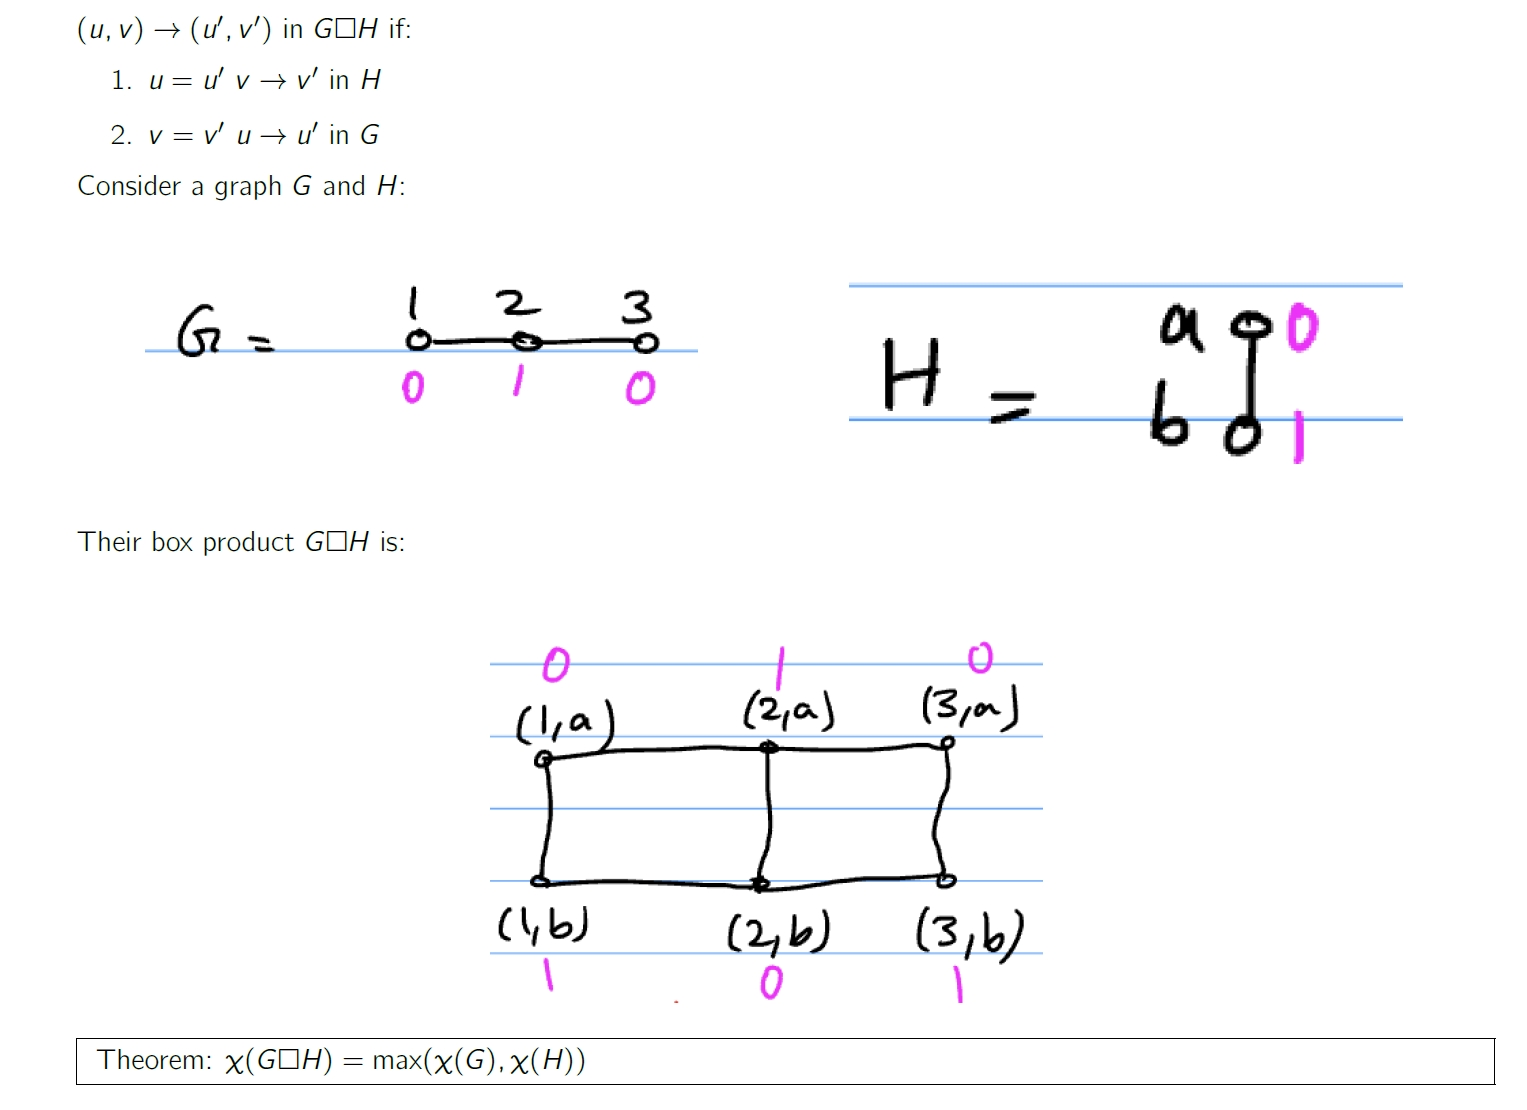
\includegraphics[scale=0.3]{Box_Product.png}
\end{center}
\section{定理/结论}
\subsection{基本结论}
$\sum_{u \in V} d(u) = 2|E|$每多一条边,$\sum d(u)$多二

Every $(u,v)$ walk contains a $(u,v)$ path.

A graph with $n$ vertices and $m$ edges has at least $n-m$ CC

$\Rightarrow$ to connect $n$ vertices, $m \geq n-1$

For $\forall v \in V$, if $d(v)\leq 2$, then $G$ is a cycle or a path.

Every connected graph with $n \geq 2$vertices has $\geq 2$ non-cut vertices.

Every odd closed walk contains an odd cycle.

if $d(i) \geq 2, \forall i \in V$ $\Rightarrow$ G has a cycle.

if $d(i) \leq 2, \forall i \in V$ $\Rightarrow$ G is a cycle or a path.
\subsection{Tree}
Tree's definition: Let $G=(V,E)$, $|V|=n$, $|E|=m$, then \\
"$G$ is connected and $m=n-1$"$\iff$"$G$ is connected and has no cycles"$\iff$ "$m = n-1$, $G$ has no cycles."

$G$ is a tree $\iff$ there is a unique path between every pair of vertices.

A connected graph $G$ is a tree $\iff$ all edges is a cut.

Adding a edge to a tree creates exactly one cycle.

Suppose $V=[n]$, then $2^{\binom{n}{2}}$ graphs exist, and $n^{n-2}$ of them are trees. This is because for every pair of vertices, there can be a edge or not have a edge, so $2^{\binom{n}{2}}$ graphs.

Every connected graph $G$ has a subgraph $T$ such that $T$ is a tree.

If $G$ is a tree, then every longest path in G is a $(u,v)$ path where both $u$ and $v$ are leafs. More about the ways to find the longest path in \ref{sec:Algo_to_longest_path}.

If $T$ is a tree with 3 or more vertices, then no leaf is a center.

Let $T$ be a tree, then $T$ either has 1 center $c$, or 2 neighbouring centers $c_{1},c_{2}$.
\subsection{Bipartite}
A graph is bipartite $\iff$ it has no odd cycle
\subsection{Special Cycles}
$G$ is Eulerian $\iff$ $d(i)$ is even for $\forall i \in V$
\subsection{Graphic}
$d_{1} \sim d_{n}$is graphic $\iff$ $d_{1}-1 \sim d_{n}-1$ is graphic.

$\because$ Every different graphic sequence corresponds to a different tree. $\therefore$ There can be $n^{n-2}$ different trees with $n$ different vertices.
\subsection{Directed Graph}
Let $G$ be a loopless directed graph, $G$ is a DAG $\iff$ $G$ is a SCC.

$G$ is a DAG $\iff$ $G$ has a topological ordering ($G$ has no loops).

In a directed $G$, if the out-degree/in-degree of every vertex is at least 1, then there's a cycle.
\subsection{Matching}
Berge Theorem: A matching $M$ is maximum $\iff$ it does not have an augmenting path.

When $M$ has an augmenting path, then $|M'| = |M|+1$ must exist.

Hall's Theorem: in a XY-bipartite graph, there's a matching $M$ saturating $X$ if and only if for$\forall S \subseteq X, |N(S)|\geq |X|$

Corollary from Hall's Theorem: Let $G$ be a $k$-regular bipartite graph. ($k$-regular means $d(v) = k,v\in V$)($k\geq 1$).$G$ has a perfect matching.
\subsection{Vertex Cover $\&$ Edge Cover}
In every graph $G$, min $|VC| \geq$ max$|M|$

K\"{o}nig's Theorem: In every bipartite graph $G$, min $|VC|=$ max $|Matching|$.

$A$ is a Vertex Cover $\iff$ $V \setminus A$ is a Independent Set.

In any graph with $|V|=n$, $\max{IS}+\min(VC)=n$

$\max{Matching}+\min{Edge Cover}=n$ for any graph with no isolated vertex.

Gallei's Theorem: In every graph $G$ without isolated vertices, max $|M|$+min$|EC|$=$n$
\subsection{Network Flow}
Max Flow Min Cut Theorem: in a directed graph G, the max flow is the capacity of all the cuts.
\subsection{Stable Matching}
Stable Matching Theorem: In a XY-bipartite graph with sizeof(X)=sizeof(Y)=n, every $x_{i},y_{i}$ has a permutation of Y and X, there's always a stable perfect matching.
\subsection{Graph Colouring}
In every graph $G$, $\chi(G) \geq \omega(G)$, i.e. the color needed to properly color $G$ is greater than the biggest clique.

$chi(G)\geq \frac{n}{\alpha(G)}$. ($\alpha(G)$ is the size of the largest Independent Set.)

Let $G$ be a graph with maximum degree $\delta$, then $\chi(G) \leq 1+\delta$

Brook's Theorem: the only graphs that need $\delta +1$ colours are odd cycles and complete graphs.\

Suppose G is a graph with degree sequence $d_{1}\geq d_{2} \geq d_{3} \geq \dots \geq d_{n}$,then $\chi(G) \leq 1+max_{i}\{min\{d_{i},i-1\}\}$

$\chi(G\Box H)=\max(\chi(G),\chi(H))$
\section{Algorithms}
\subsection{Maximum Spanning Tree}
\subsubsection{Kruskal's algorithm}
sort edges by increasing weight, if choosing the smallest-weight edge that is not in MST creates a cycle, then discard it, if not, then take it into MST.
\subsubsection{Prim's algorithm}
start from any vertex $u$, take the smallest-weight edge from $u \in MST$ to a new vertex not inside MST.

\subsection{Finding the Maximum Independent Set for $G$ is a tree}
pick any arbitrary $v$ as root, let $T_{v}$ be a subtree of $T$ rooted at $v$.

$is_{0}[v] = $the size of the largest IS such that $v \notin I$

$is_{1}[v] = $the size of the largest IS such that $v \in I$

if $l$ is a leaf, then $is_{0}[l] = 0;is_{1}[l] = 1$,

if $l$ isn't a leaf, then $is_{0}[l] = \sum_{c_{i}}(max\{is_{0}[c_{i}], is_{1}[c_{i}]\});\; is_{1}[l] = \sum_{c_{i}}(is_{0}[c_{i}])+1$

output = $max\{is_{0}[r],is_{1}[r]\}$

\subsection{Algorithm to find the longest path} \label{sec:Algo_to_longest_path}
$depth[v] = 1+max\{depth[c_{i},c_{i}$ is $v$'s children$\}$($v$ is not a leaf) or $depth[v] = 0$($v$ is a leaf)

define $lp[v] = $length of the longest path whose highest depth is $v$.

$lp[v] = max\{depth[v],2+max\{c_{i}\}+max\{c_{j}\}\}$($i \neq j$)

\subsection{Path length calculation}
Define $\alpha(u,v,k)$ as 1 if there is a walk with $k$ edges from $u$ to $v$, otherwise 0. then $d(u,v)$ is the smallest $k$ such that $\alpha(u,v,k)=1$.

$\alpha(u,v,k) = \bigvee_{w\in N(v)} \alpha(u,w,k-1)$, $\alpha(u,u,0)=1, \alpha(u,v,0)=0$ for $u \neq v$

\subsection{Dijkastra's Algorithm}
(To find a minimum path from $u$ to $v$ in a non-negative weighted graph)——贪心算法和广度优先的结合

1.从起始点$u$开始计算所有和它相连的点(也就是起始点指向的点),计算完之后把起始点标记下(表示已经计算过了)。

2.找出离起始点最近且没有被标记过的点$v$,计算所有和$v$相连且没有被标记过的点,计算完之后把$v$标记下。即:For each neighbor $n$ of $v$, if($d(u,v)+w(v,n)>d(u,n)$), then update $d(u,w)=d(u,v)+w(v,n)$

3.重复上面的步骤2.直到所有顶点都标记完为止。

\subsection{Ford-Fulkerson's algorithm}
First initialize all $f$ to 0, then find any path from $s$ to $t$ such that every edge in the path is either non-full forward or non-empty backwards. Add to each edge of the path until there's a edge that's empty or full. Repeat.\\

\noindent Greedy Colouring: pick any order for colouring, when colouring vertex $i$, assign the smallest colour number $j$ that's not in its neighbours.
\section{重要定理证明}
\noindent Hall's Theorem:\\$\indent$
"$\Rightarrow$": $\because$ It's a matching, $\therefore$ there must be at least one vertex in $Y$ that is a neighbour of a vertex in $X$, $|N(S)|\geq |S|$

"$\Leftarrow$": 取逆否命题,即原命题的反命题:To proof="if maximum matching $M$ does not saturate $X$, then $|N(S)|<|S|$"

$\exists x_{0}\in X, x_{0}\notin M.$ Set $x_{1} \sim x_{n} \in X\cap M = \overline{X}, y_{1} \sim y_{n} \in Y\cap M = \overline{Y}$

a) Proof $x_{0}$'s neighbour is in $\overline{Y}$: if $x_{0}$'s neighbour $\in Y\setminus\overline{Y}$, then count that edge into $M$, contradicting to $x_{0} \notin M$.

b) Proof $\forall x \in \overline{X}, \nexists v\in Y\setminus\overline{Y}$ such that $(x,v)$ is a edge: if so, then $x_{0}, y_{i_{1}}, x_{i_{1}}, y_{i_{2}}, x_{i_{2}}, \dots, y_{i_{n}}, x, v$ is a augmenting path, contradicting to $M$ is a maximum matching.

$\Rightarrow$ $|N(S)| = |\overline{Y}| = |S|-1 < |S|$得证.
\section{方法}
In a game consisting of two players, consider assigning a label to every state of the game.

To proof something exists, construct a algorithm that has a termination proof and a correctness proof.

\ifdebug
\end{document}
\fi